\chapterimage{chapter_head_2.pdf} % Chapter heading image

\chapter{Recommended Software}
By the time you read this, it will be out of date!  A colleague of mine used to say ``computers are our microscopes", when comparing psychological science to other fields like biology. The advancement of technology, including hardware and software, has quite literally provided a scaffolding for research in the field of psychological science.  While advancements in computer hardware have revolutionized methods of control in psychological experiments and opportunities for new analyses, advancements in software continue to open new doors to research techniques, make analytic methods available to everyone, support replicability, and improve communication.

In this chapter, you will find introductions to a number of software applications that I have found particularly useful in my teaching and research.
\newpage

%------------------------------------------------
\section{Zoom}\index{Zoom}
Zoom is a free, web-based and/or desktop application for online video conferencing.  We will be using Zoom for lecture delivery, lab meetings, and office hours.
\subsection{Installation}\index{Installation}
\reversemarginpar
\marginnote{\begin{pspicture}(20mm,20mm)
        \psbarcode{https://zoom.us/download}{eclevel=H width=.35 height=.35}{qrcode}
        \end{pspicture}}[-1cm]
Zoom can be run using either just a web browser, or using their desktop application. The \textbf{recommended} method for using Zoom in this class is to download the desktop application from \weblink{https://zoom.us/download}.  Once installed, all you need to do is open the application and log in using your William \& Mary credentials.
\normalmarginpar\marginnote{\footnotesize{\textcolor{orange}{Note that there are Zoom apps for iOS, Chrome OS, and Android devices too!}}}[-1cm]

To use a web browser, simply visit \weblink{https://cwm.zoom.com} and log in using your William \& Mary credentials.  Once you have logged in, you will be able to configure the appropriate settings.
\reversemarginpar\marginnote{\begin{pspicture}(25mm,25mm)
        \psbarcode{https://cwm.zoom.com}{eclevel=H width=.35 height=.35}{qrcode}
        \end{pspicture}}[-2.5cm]


\subsection{Recommended Settings}\index{Zoom Settings}
Zoom is highly configurable, with many settings under the users control. Below are just a few recommended settings that can help to ensure smooth multi-user meetings!

    \begin{wrapfigure}[10]{r}{0.39\textwidth}
    \centering
    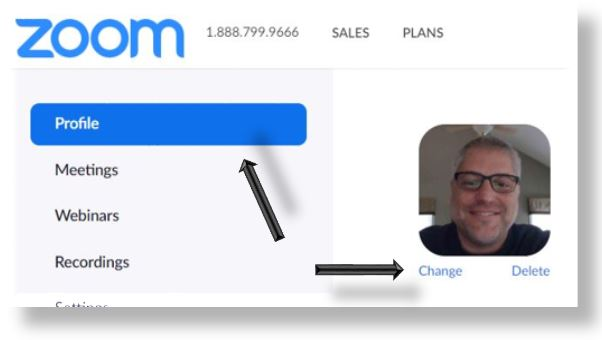
\includegraphics[scale=0.45]{zoom1.jpg}
    \caption{Zoom profile}
    \label{fig:zoom1}
    \end{wrapfigure}
\noindent    
\subsubsection{Profile}
Personalize your profile image! In the desktop application, click the settings (gear icon) button and select \texttt{Profile} $\rightarrow$ \texttt{Edit My Profile}.  If logged into the Zoom website, select \texttt{Profile} from the links on the left and then click the change link beneath your current profile image (see Figure \ref{fig:zoom1}).

\subsubsection{Audio}
It is important to set up your Zoom account so that your audio is muted by default.  There is also an option to that will allow you to enact a push-to-talk. This feature allows you to use your microphone temporarily by pressing and holding a bound-key on your computer (e.g., the spacebar; see Figure \ref{fig:zoom2}).
    \begin{figure}[h]
    \centering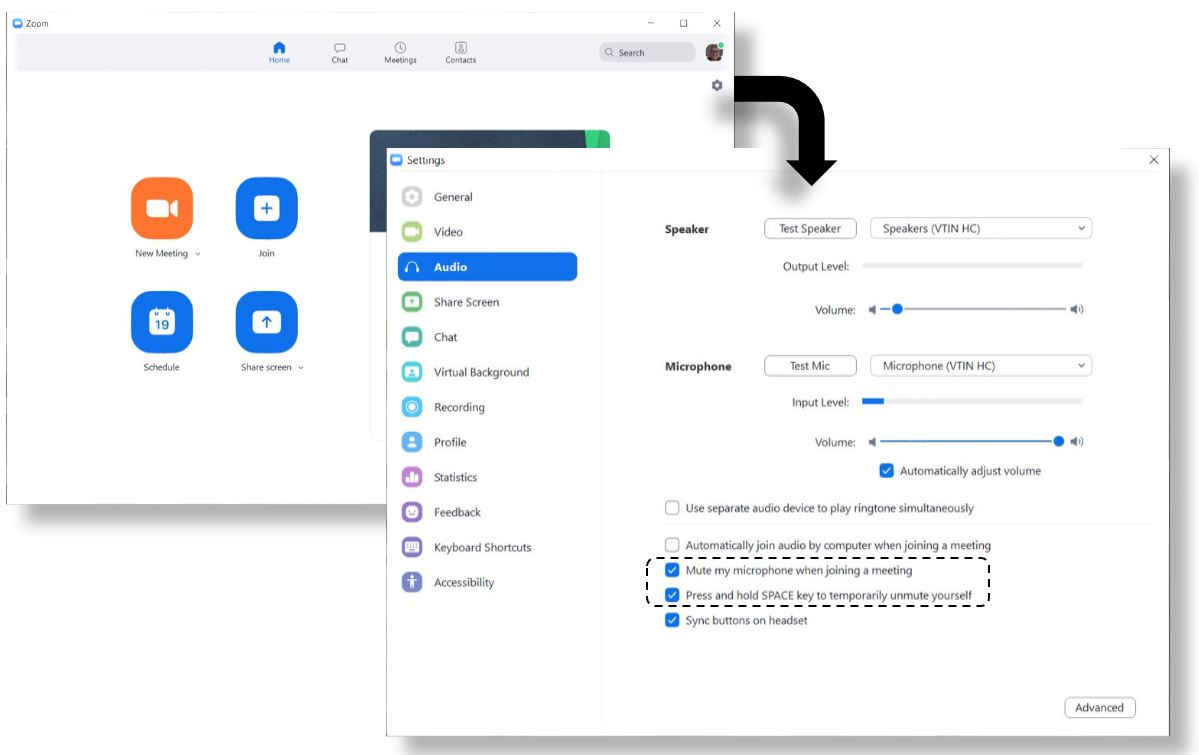
\includegraphics[scale=0.4]{zoomdesktopaudio.jpg}
    \caption{Zoom audio settings}
    \label{fig:zoom2}
    \end{figure}

\subsection{Other Useful Features}
Zoom possesses a number of tools that can facilitate communication in meetings, most of these tools are available to both participants and host(s) of the meetings.  A few of these tools are described below.
\subsubsection{Push-to-Talk}
    Assuming the audio settings are configured as described above, the microphone of all meeting attendees will be muted by default. This is especially helpful in reducing background noise in larger meetings (e.g., >10), which can make it difficult to hear any one speaker in the conversation/presentation.  When an attendee does wish to contribute they can simply hold the space bar down to un-mute the microphone while speaking and release the space bar to re-mute the microphone.
\subsubsection{Screen Sharing}
    Screen sharing is useful for presentations, allowing all participants in the meeting to view the same screen content (e.g., Power Point or Google Slides). Screen sharing can also be configured in settings (gear icon) to display both the shared screen \textit{and} the feed(s) from the participant(s) camera.  There is also a ``whiteboard" option that allows for free form drawing using the cursor or digital pen.    
\subsubsection{Raise Your Hand}
    While Zoom offers a nice interface for large group meetings with a Brady-Bunch style tiling of participants camera feeds, there are cases in which the meeting host might like to present their screen (e.g., f slides) to all participants and may not be aware when there are questions or comments from other participants.  Fortunately, participants (but not hosts) have a ''raise your hand" option when they click the "Participants" button that is part of the Zoom controls when logged into a meeting.  Even when presenting a window in full-screen to participants, the hose will receive an alert when the ''raise your hand" button is clicked by any participant, providing an opportunity to pause the presentation and solicit feedback from meeting participants.
\subsubsection{Annotation Tools}
    Another really useful tool in Zoom is the annotation toolbar.  The toolbar can be made available by clicking the ``Annotate" button in Zoom, whenever the host (or participant) is presenting their screen to the group.  For hosts, the "Spotlight" tool works like a laser pointer that can be used to highlight portions of the screen during a presentation.  Other tools, like "Text" and "Draw" can be useful for participants to make comments or draw attention to a portion of the screen when there are questions during a presentation.  Note, however, that these text and drawing comments are persistent and will need to be erased by the host using the ``Clear" button on the Annotations toolbar when advancing to the next slide (see Figure \ref{fig:zoomannotate}).
    \begin{figure}[h]
    \centering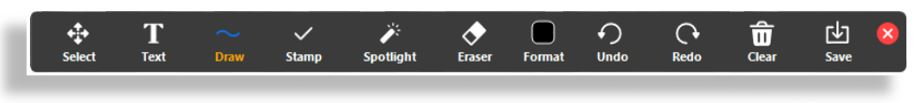
\includegraphics[scale=0.7]{zoomannotate.jpg}
    \caption{Zoom annotation tools}
    \label{fig:zoomannotate}
    \end{figure}
\subsubsection{Chat}
    Zoom also has a ``chat" feature that permits both public and private messaging between participants.  Parameters of the chat permissions are accessible in the ``Chat" panel of the settings (gear icon) menu in Zoom.  Private chats between participants can also be disabled (recommended for webinar/classroom uses).
\subsubsection{Remote Control}
    Remote control is actually one of the "Screen share" options in Zoom. Enabling \texttt{remote control of all operations} can be especially useful in courses that require heavy use of computer applications.  If the situation requires, students can grant you (as the host) control over their computer, meaning that you can use your cursor to control the operation of their computer remotely.  This can be used to demonstrate procedures, install software, etc.
\subsubsection{Scheduling Meetings}
    Meetings can be created ``on the fly" or can be scheduled in advance.  Each meeting is assigned either a unique meeting ID number or your personal meeting ID number (linked to your Zoom account). The meeting ID number determines how participants will access the meeting so an advantage of using your personal ID number is that invited participants will have access the current and any future meeting you host, without the need to repeatedly provide meeting access information (e.g., web links, meeting ID, etc.). You can also set up ``recurring" meetings in Zoom.  Similar to setting up a meeting using your personal ID, these recurring meetings will use a persistent meeting ID number. 
    
    Note that if you configure your recurring Zoom meeting to enable ``join before host", you will effectively have created a persistent virtual meeting room in which participants can interact (even without the meeting host) at any time of day/night.
    

%------------------------------------------------
